\documentclass[11pt]{article}
\usepackage[margin=0.72in]{geometry}
\usepackage{amsmath,amssymb,booktabs,tabularx,longtable,array}
\usepackage{graphicx,float,caption}
\usepackage[dvipsnames]{xcolor}
\usepackage{hyperref}
\usepackage{listings}
\usepackage{fancyhdr}
\usepackage{microtype}
\usepackage{enumitem}
\usepackage{tikz}
\usetikzlibrary{arrows.meta,positioning,shapes.geometric}

\definecolor{Navy}{HTML}{183B5B}
\definecolor{Teal}{HTML}{168B8B}
\definecolor{Orange}{HTML}{D98200}
\definecolor{Red}{HTML}{B33430}
\definecolor{Pale}{HTML}{EFF5F8}
\hypersetup{colorlinks=true,linkcolor=Navy,citecolor=Teal,urlcolor=Navy}
\pagestyle{fancy}
\fancyhf{}
\lhead{NeuroKit default gradient detector}
\rhead{audited implementation: NeuroKit2 0.2.13}
\cfoot{\thepage}
\setlength{\headheight}{14pt}
\setlist[itemize]{leftmargin=1.5em,itemsep=2pt}
\setlist[enumerate]{leftmargin=1.7em,itemsep=3pt}
\newcolumntype{Y}{>{\raggedright\arraybackslash}X}
\newcommand{\important}[1]{\begin{center}\fcolorbox{Red}{red!4}{\parbox{0.93\linewidth}{\textbf{\color{Red}#1}}}\end{center}}
\newcommand{\levelbox}[2]{\begin{center}\fcolorbox{#1}{Pale}{\parbox{0.93\linewidth}{#2}}\end{center}}
\lstset{basicstyle=\ttfamily\footnotesize,backgroundcolor=\color{Pale},frame=single,breaklines=true,columns=fullflexible,showstringspaces=false}

\title{\textbf{NeuroKit's Default Gradient R-Peak Detector, Step by Step}\\
\large Child-level intuition, programmer-level implementation, professor-level audit,\\
and literal outputs from the local MIT--BIH data}
\author{RR--HRV cascade implementation report}
\date{5 August 2026}

\begin{document}
\maketitle

\important{NeuroKit's default method is a useful software algorithm, but its default detector is not a separately published named method.  NeuroKit2 itself is published and validated as a toolbox \cite{makowski2021neurokit}; the exact gradient-region/local-prominence logic and its default parameters are documented in the official source \cite{neurokitpeaksource}.  Claims about how the default works must therefore cite the source code, and claims about performance must cite an explicit benchmark or this audit.}

\section*{What was actually audited}
The local diagnostic script copied the inspected NeuroKit2 0.2.13 operations into transparent stages and required the final sample array to equal \texttt{nk.ecg\_findpeaks(cleaned, method="neurokit")} exactly.  On record 108, both contained 1,744 samples.  The separate project wrapper with an experimental 250-ms inclusive delay produced 1,749; it is not the library default.

\begin{table}[H]
\centering
\caption{Four different questions that are often confused.}
\begin{tabularx}{\linewidth}{@{}p{0.26\linewidth}YY@{}}
\toprule
Question & What NeuroKit does & What it does not establish \\
\midrule
Is there steep QRS-like activity? & Uses the absolute ECG gradient and an adaptive local threshold to create candidate regions. & A region can also arise from a steep T wave, pacing spike or artifact. \\
Where is a positive peak inside it? & Chooses the positive local maximum with greatest prominence. & It does not test whether a negative extremum is the better fiducial. \\
Is it sufficiently separated? & Default accepts only if more than 300 ms after the previous accepted peak. & This is not a clinical proof that two closer QRS complexes are impossible. \\
Is it a true beat? & Benchmarking against expert annotations can answer this retrospectively. & The detector itself does not output beat class, artifact probability or seizure probability. \\
\bottomrule
\end{tabularx}
\end{table}

\clearpage
\section{The whole timeline in one view}
\begin{figure}[H]
\centering
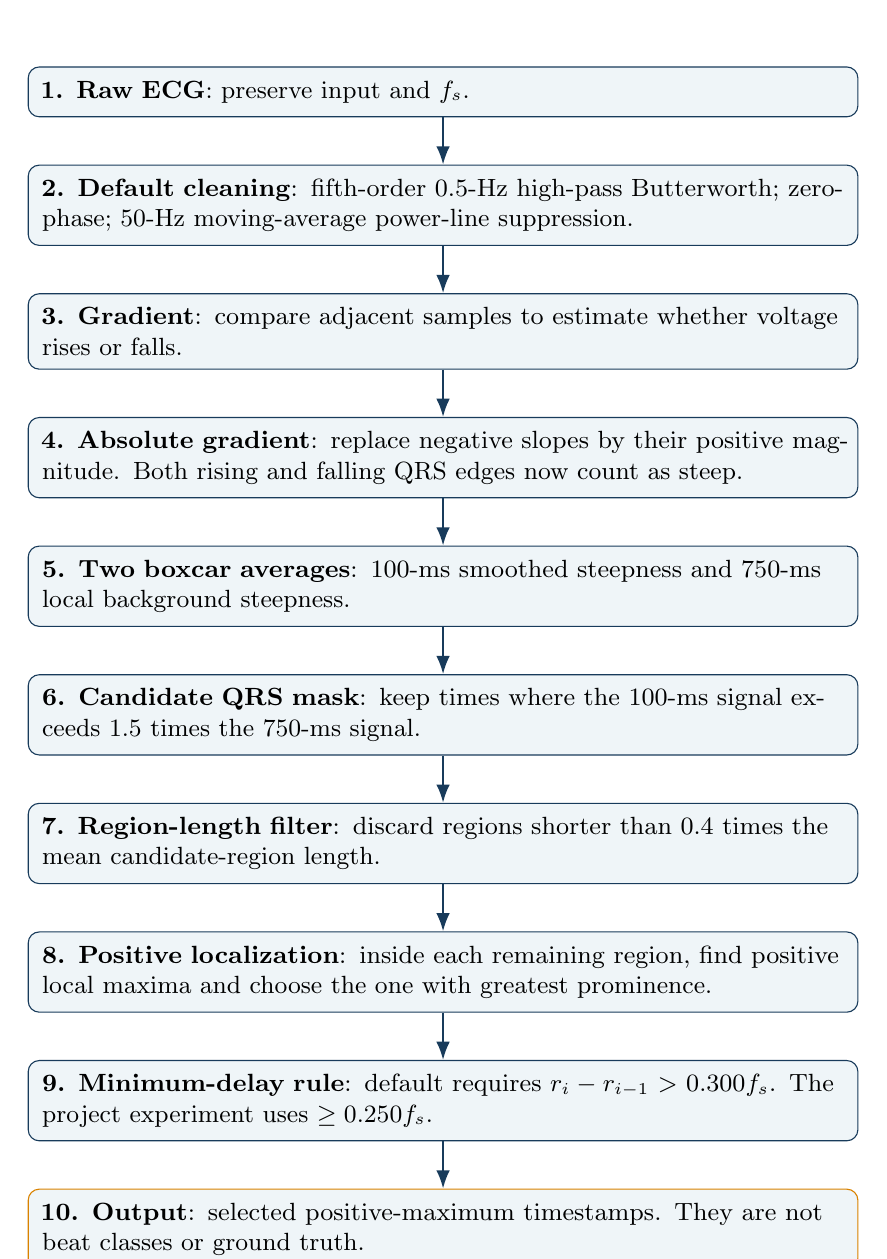
\begin{tikzpicture}[node distance=6mm,>=Latex,
box/.style={draw=Navy,rounded corners,fill=Pale,text width=0.84\linewidth,align=left,inner sep=5pt,font=\small},
arr/.style={->,thick,Navy}]
\node[box] (a) {\textbf{1. Raw ECG}: preserve input and \(f_s\).};
\node[box,below=of a] (b) {\textbf{2. Default cleaning}: fifth-order 0.5-Hz high-pass Butterworth; zero-phase; 50-Hz moving-average power-line suppression.};
\node[box,below=of b] (c) {\textbf{3. Gradient}: compare adjacent samples to estimate whether voltage rises or falls.};
\node[box,below=of c] (d) {\textbf{4. Absolute gradient}: replace negative slopes by their positive magnitude. Both rising and falling QRS edges now count as steep.};
\node[box,below=of d] (e) {\textbf{5. Two boxcar averages}: 100-ms smoothed steepness and 750-ms local background steepness.};
\node[box,below=of e] (f) {\textbf{6. Candidate QRS mask}: keep times where the 100-ms signal exceeds \(1.5\) times the 750-ms signal.};
\node[box,below=of f] (g) {\textbf{7. Region-length filter}: discard regions shorter than \(0.4\) times the mean candidate-region length.};
\node[box,below=of g] (h) {\textbf{8. Positive localization}: inside each remaining region, find positive local maxima and choose the one with greatest prominence.};
\node[box,below=of h] (i) {\textbf{9. Minimum-delay rule}: default requires \(r_i-r_{i-1}>0.300f_s\). The project experiment uses \(\ge0.250f_s\).};
\node[box,below=of i,draw=Orange] (j) {\textbf{10. Output}: selected positive-maximum timestamps. They are not beat classes or ground truth.};
\foreach \u/\v in {a/b,b/c,c/d,d/e,e/f,f/g,g/h,h/i,i/j}{\draw[arr] (\u)--(\v);}
\end{tikzpicture}
\caption{Exact processing order of the inspected default implementation \cite{neurokitcleaningsource,neurokitpeaksource}.}
\end{figure}

\clearpage
\section{Explain it to a child}
\levelbox{Teal}{\textbf{The steep-slide story.} Draw the ECG as a roller-coaster.  A QRS is often the part where the track rises or falls very quickly.  NeuroKit measures how steep the track is.  It turns both ``steep up'' and ``steep down'' into positive numbers, then smooths them so one heartbeat makes one wide bright zone.  Inside the zone it looks back at the cleaned ECG and chooses the most noticeable \emph{positive hilltop}.}

The word ``gradient'' just means local change.  With samples (x[n-1],x[n],x[n+1]), NumPy's interior approximation is
\[
g[n]\approx\frac{x[n+1]-x[n-1]}{2}.
\]
If the right-hand sample is higher, the gradient is positive. If it is lower, the gradient is negative. The absolute gradient (|g[n]|) asks only ``how steep?''

\begin{figure}[H]
\centering
\includegraphics[width=\linewidth]{figures/neurokit_record108_j_transformations.png}
\caption{Literal transformation of the expert (j) beat at sample 435,657 in MIT--BIH record 108.  The region detector sees both QRS edges, but the final localization stage allows positive local maxima to compete.}
\end{figure}

\important{NeuroKit is partly polarity-insensitive and partly polarity-sensitive: absolute gradient finds steep activity in either direction, but the final positive-maximum search can neglect a dominant negative QRS trough.}

\clearpage
\section{Explain it to a programmer: default cleaning}
For \texttt{ecg\_clean(method="neurokit")}, the inspected source applies:
\begin{enumerate}
\item a fifth-order Butterworth high-pass filter at 0.5 Hz using zero-phase forward/backward filtering;
\item power-line suppression using a moving average one nominal 50-Hz period long.
\end{enumerate}
At 360 Hz, \texttt{int(360/50)=7} samples.  This is a seven-sample moving average in the local environment, not a universal notch-filter implementation.  Exact preprocessing should be version-locked because detector inputs are not interchangeable \cite{neurokitcleaningsource}.

\begin{lstlisting}[caption={Audited preprocessing skeleton.}]
cleaned = nk.ecg_clean(raw, sampling_rate=360, method="neurokit")
# Internally in the inspected version:
# high-pass Butterworth, order 5, cutoff 0.5 Hz, zero phase
# power-line moving average, default line frequency 50 Hz -> 7 samples
\end{lstlisting}

\begin{table}[H]
\centering
\caption{Literal default parameters at 360 Hz.}
\begin{tabularx}{\linewidth}{@{}lrrY@{}}
\toprule
Parameter & Time/frequency & Samples & Role \\
\midrule
High-pass cutoff & 0.5 Hz & --- & Reduce baseline drift. \\
Power-line period & 20 ms at 50 Hz & 7 & Moving-average suppression in inspected code. \\
Gradient smoother & 100 ms & 36 & Merge edge-by-edge steepness into QRS evidence. \\
Background average & 750 ms & 270 & Provide a local adaptive reference. \\
Threshold weight & \(1.5\times\) & --- & Candidate mask comparison. \\
Minimum length weight & \(0.4\times\) mean & --- & Reject very brief candidate regions. \\
Minimum accepted delay & \(>300\) ms & 108 & Prevent accepted events from being too close. \\
\bottomrule
\end{tabularx}
\end{table}

\clearpage
\section{Explain it to a programmer: gradient and threshold}
Let \(c[n]\) be the cleaned ECG.
\[
g[n]=\operatorname{gradient}(c)[n],\qquad a[n]=|g[n]|.
\]
The code performs boxcar smoothing:
\[
s_{100}[n]=\operatorname{mean}_{100\mathrm{ms}}a[n],\qquad
m_{750}[n]=\operatorname{mean}_{750\mathrm{ms}}s_{100}[n].
\]
The time-varying threshold and mask are
\[
\tau[n]=1.5m_{750}[n],\qquad M[n]=\mathbb{1}\{s_{100}[n]>\tau[n]\}.
\]
Each contiguous true run of \(M[n]\) is a candidate region.  In record 108 there were 2,260 threshold regions, mean length 42.44 samples, and the minimum retained length was \(0.4\times42.44=16.98\) samples.  Candidate count is not peak count: many regions are short or later blocked.

\begin{table}[H]
\centering
\caption{Plain-language interpretation of each transformation.}
\begin{tabularx}{\linewidth}{@{}p{0.19\linewidth}p{0.22\linewidth}Y@{}}
\toprule
Object & Mathematical question & Plain meaning \\
\midrule
\(g[n]\) & Direction and amount of sample-to-sample change & Is the trace going up or down, and how rapidly? \\
\(|g[n]|\) & Magnitude only & Treat steep up and steep down as equally interesting. \\
\(s_{100}[n]\) & Short-term average steepness & Is this neighborhood QRS-like rather than a one-sample flicker? \\
\(m_{750}[n]\) & Longer local average & How much steepness is ordinary around here? \\
\(s_{100}>1.5m_{750}\) & Relative excess & Is this neighborhood substantially steeper than its recent context? \\
\bottomrule
\end{tabularx}
\end{table}

\important{An adaptive threshold reduces sensitivity to absolute voltage scale, but it does not know cardiac anatomy. Any sufficiently steep non-QRS deflection can create a candidate region.}

\clearpage
\section{Explain it to a programmer: prominence and timing}
Inside each retained region, SciPy \texttt{find\_peaks} enumerates \emph{positive} local maxima.  The algorithm chooses the maximum with greatest prominence.

\subsection{What is prominence?}
Imagine flooding the ECG landscape from below.  A hill's prominence is how far its summit stands above the highest surrounding saddle needed to reach a taller hill.  A tall bump riding on an already high shoulder can be less prominent than a slightly lower isolated bump.  Prominence therefore is not identical to absolute amplitude.

Formally, if peak \(p\) has surrounding reference level \(b_p\), then
\[
\operatorname{prominence}(p)=c[p]-b_p.
\]
The exact base-search rules are supplied by SciPy; NeuroKit uses the returned prominences and selects \texttt{argmax(prominences)} \cite{neurokitpeaksource}.

For the record-108 expert \(j\) beat, the candidate region ran from sample 435,628 to 435,685: 57 samples or 158.3 ms.  It contained one positive local maximum.  NeuroKit selected sample 435,656, 2.78 ms before the expert sample 435,657; cleaned amplitude was 0.6737 mV and prominence 0.7054 mV.

\begin{lstlisting}[caption={Exact decision pattern in the inspected source.}]
local_maxima, properties = scipy.signal.find_peaks(
    cleaned[begin:end], prominence=(None, None)
)
candidate = begin + local_maxima[argmax(properties["prominences"])]
if candidate - previous_accepted > round(0.300 * fs):
    accept(candidate)
\end{lstlisting}

The default strict greater-than comparison matters. At 360 Hz, 300 ms is 108 samples. A candidate exactly 108 samples after the previous accepted event fails because \(108>108\) is false.

\clearpage
\section{Minimum delay, tachycardia and bradycardia}
For consecutive R timestamps,
\[
RR_{\mathrm{ms}}=1000\frac{r_i-r_{i-1}}{f_s},\qquad
BPM=\frac{60,000}{RR_{\mathrm{ms}}}=60\frac{f_s}{r_i-r_{i-1}}.
\]
Therefore 300 ms corresponds to \(60{,}000/300=200\) bpm, and 250 ms corresponds to 240 bpm.  These are instantaneous interval conversions, not claims about clinical rhythm diagnosis.  Adult resting tachycardia is often described above 100 bpm, but that does not imply ordinary QRS detectors fail at 101 bpm; the software's hard timing ceiling appears only near its minimum-delay boundary.

\begin{figure}[H]
\centering
\includegraphics[width=0.96\linewidth]{figures/neurokit_minimum_delay_timeline.png}
\caption{Direct mathematical effect of the minimum-delay setting.  The original source requires strictly more than 300 ms; the project experiment uses at least 250 ms.}
\end{figure}

\subsection{Can it detect bradycardia?}
The minimum delay does not block long intervals, so bradycardia is not rejected merely because RR is long.  However, the 750-ms local threshold and recording boundaries can affect region formation; missing a low-amplitude beat can make an interval falsely long.

\subsection{Can it detect tachycardia?}
It can detect rates well above 100 bpm.  With the default rule, candidates separated by 400 ms (150 bpm) remain eligible. At exactly 300 ms the strict test fails; below it, every second event may be blocked depending on candidates.  Lowering the delay to 250 ms expands eligibility but also admits more T waves, fragmented QRS peaks and noise.  The local all-48 audit found this trade-off rather than a free improvement.

\clearpage
\section{Professor-level audit: why record 113 fails}
Record 113 is a crucial counterexample because expert metadata describes predominantly normal sinus rhythm, yet the default NeuroKit output contains many extra detections.  Under the local \(\pm75\)-ms expert matching audit, NeuroKit found 1,794 true positives, 1,039 false positives and one false negative.  The repeated false candidates occurred roughly 303--372 ms after true QRS events; the displayed example is 316.7 ms later.

\begin{figure}[H]
\centering
\includegraphics[width=\linewidth]{figures/neurokit_record113_twave_double_detection.png}
\caption{A literal record-113 example.  The post-QRS deflection is steep enough to form its own region, contains a positive maximum and appears 316.7 ms after the previous accepted QRS---just beyond the default delay.  Timing and shape are consistent with T-wave double detection, but the \texttt{.atr} file does not label T waves; the identity is therefore an informed morphological inference, not annotation ground truth.}
\end{figure}

The failure follows directly from the algorithm:
\begin{enumerate}
\item the post-QRS/T-wave deflection has steep rising and falling edges;
\item absolute gradient makes both positive;
\item smoothed steepness crosses the adaptive threshold;
\item the region is not too short;
\item the region contains a prominent positive maximum;
\item 316.7 ms is strictly greater than 300 ms, so the delay rule permits it.
\end{enumerate}
This is detector error on a largely clean signal, not evidence of physical artifact.  It also shows why reducing the delay to 250 ms cannot solve this case; it only makes the time test more permissive.

\clearpage
\section{Professor-level audit: polarity and the missing negative choice}
The early detector is approximately polarity-neutral:
\[
|\nabla(-c)|=|-\nabla c|=|\nabla c|.
\]
The final localizer is not:
\[
r_i^{NK}=\underset{p\in\text{positive local maxima in region}}{\arg\max}
\operatorname{prominence}(p).
\]
For a predominantly negative QRS, the most physiologically stable fiducial may be a deep trough, yet the candidate set excludes troughs.  The algorithm can select a small positive shoulder, a nearby rebound or nothing.

\subsection{Does NeuroKit already have automatic inversion?}
NeuroKit provides an ECG inversion utility, but calling it is a separate decision.  The default peak-finder does not automatically compare positive and negative fiducials inside each QRS and select the clinically correct one.  Running the complete detector on (x) and (-x) creates two candidate streams; our current pipeline stores the inverted stream as diagnostic context and allows the original stream to own RR.  There is no automatic branch router in the current implementation.

\subsection{Why not choose whichever has larger amplitude?}
Absolute amplitude can prefer a deep S wave over an R wave, a pacing spike over ventricular depolarization, or an artifact over either.  The term ``R peak'' in an annotation database is a fiducial convention tied to QRS morphology, not simply the largest absolute voltage in a 100-ms box.  PhysioZoo's \texttt{qrs\_adjust} still requires a sign input, and R-DECO provides positive/negative templates plus visual correction \cite{physiozooqrsadjust,rdeco2021}.  These precedents support separating event detection from fiducial localization; they do not supply a universal beat-wise sign oracle.

\important{Detector agreement does not settle polarity. Two algorithms can agree that a QRS occurred while reporting different edges/extrema. The agreement is evidence for the event, not proof that either timestamp is the correct R fiducial.}

\clearpage
\section{Literal benchmark outputs}
All 48 MIT--BIH records were evaluated against expert beat annotations \cite{goldberger2000physiobank,moody2001mitbih,physionetmitdb}.  The same \(\pm75\)-ms event-matching rule was used for both configurations.

\begin{table}[H]
\centering
\caption{Local all-record audit of default and experimental delay.}
\begin{tabular}{@{}lrrrrrr@{}}
\toprule
Configuration & TP & FP & FN & Sensitivity & PPV & \(F_1\) \\
\midrule
Default \(>300\) ms & 107,677 & 2,503 & 1,817 & 0.98341 & 0.97728 & 0.98033 \\
Project \(\ge250\) ms & 107,713 & 2,780 & 1,781 & 0.98373 & 0.97484 & 0.97927 \\
\bottomrule
\end{tabular}
\end{table}
The shorter delay recovered 36 true beats and reduced false negatives by 36, but added 277 false positives.  Pooled F1 fell slightly.  This does not prove 250 ms is always worse; it proves the current all-record data do not support promoting it as a free improvement.  Heart-rate-stratified and target-patient validation remain necessary.

\paragraph{Notebook-style reproducibility output.}
\begin{lstlisting}
software: neurokit2=0.2.13, scipy=1.17.0
record=108, fs=360 Hz
official default count=1744
exact diagnostic reproduction count=1744
arrays exactly equal=True
expert j=435657
candidate region=[435628, 435685), length=57 samples=158.333 ms
positive local maxima=1
selected=435656, error=-2.7778 ms, prominence=0.70538 mV
previous accepted separation=1605.556 ms; passes >300 ms=True
\end{lstlisting}

\clearpage
\section{Alternatives: what problem does each solve?}
\begin{longtable}{@{}p{0.22\linewidth}p{0.32\linewidth}p{0.38\linewidth}@{}}
\caption{Literature-backed alternatives and their limits.}\\
\toprule
Alternative & Why it may help & Critical limitation / required validation \\
\midrule
\endfirsthead
\toprule
Alternative & Why it may help & Critical limitation / required validation \\
\midrule
\endhead
UNSW/Khamis primary & Published amplitude--derivative detector designed for poorer-quality telehealth ECG; strong benchmark performance \cite{khamis2016telehealth,kristof2024qrs}. & Returns QRS-event locations in a transformed signal; exact R localization remains separate. \\
PhysioZoo adjustment & Makes the QRS-to-fiducial step explicit and can search for a maximum or minimum \cite{behar2018physiozoo,physiozooqrsadjust}. & Requires the correct sign; does not automatically solve within-record polarity changes. \\
R-DECO & Envelope-based detector, positive/negative templates and manual visual correction; suitable for building a patient-specific reference set \cite{rdeco2021}. & Manual editing cannot be silently presented as deployable automation. \\
Polarity + sample-precise CNN & Explicitly separates polarity classification from sample-level localization \cite{oudkerkpool2021rpeak}. & Training burden, domain shift and failure on unusual morphologies; must be tested chronologically on the target patient. \\
Timing-aware detector comparison & JF/narrow-tolerance evaluation penalizes temporal jitter hidden by broad event windows \cite{porr2024jitter,reklewski2026noise}. & Evaluation method, not itself a detector. \\
\bottomrule
\end{longtable}

\section{Implementation decision for the RR--HRV branch}
\begin{enumerate}
\item Keep the unmodified 300-ms NeuroKit detector as the software baseline and independent secondary context.
\item Keep the 250-ms version as a named experimental ablation; do not merge its metrics with the default.
\item Do not use NeuroKit disagreement as ``artifact.''  It can represent noise, T-wave double detection, morphology, polarity or timing differences.
\item Do not use NeuroKit as a hard veto on primary UNSW events.  The prior gate audit removed real beats in difficult morphologies.
\item Report event sensitivity/PPV/F1, narrow-tolerance timing errors, RR error and morphology/rate strata separately.
\item Preserve original and inverted candidates, but do not average or automatically choose between them until a rule is validated on manually annotated target-patient ECG.
\end{enumerate}

\important{PI verdict: NeuroKit is useful as a complementary gradient-based lens and a strong baseline, not as unquestioned R-fiducial truth. Its absolute-gradient region detector and positive-prominence localizer must be discussed as separate stages because polarity robustness is lost at the second stage.}

\section*{Reproduction files}
Figures and numbers were generated by \texttt{generate\_algorithm\_explainer\_assets.py}. Literal outputs are stored in \texttt{outputs/neurokit\_literal\_outputs.json}; pooled metrics were read from the existing all-48 audit. The diagnostic implementation raises an exception if its output differs from the installed NeuroKit function.

\bibliographystyle{unsrt}
\bibliography{algorithm_explainers}
\end{document}
